\documentclass[]{article}
\usepackage[spanish.mexico]{babel}
\usepackage[T1]{fontenc}
\usepackage[utf8]{inputenc}
\usepackage{lmodern}
\usepackage[a4paper]{geometry}

%\usepackage{natbib}
\usepackage{cite}


%Grafico de barras
\usepackage{pgfplots}

%Graficos e imagenes
\usepackage{graphicx}

%URL
\usepackage{hyperref}



%\title{Proyecto de Optimización de Energía}
%\author{Pablo Vivar Colina}
%\date{Mayo 2018}

%\usepackage[top=2cm,bottom=2cm,left=1cm,right=1cm]{geometry}


\begin{titlepage}
     \begin{center}
	
\includegraphics[width=0.09\textwidth]{UNAM}\Large Universidad Nacional Autónoma de México
        	
\includegraphics[width=0.09\textwidth]{FI}\\[1cm]
        \Large Facultad de Ingeniería\\[1cm]
       % \Large División de Ciencias Básicas\\[1cm]
         \Large Laboratorio de Fundamentos de Control(6655)\\[1cm]
         %la clave antes era:4314
         \footnotesize Profesor: Salcedo Ubilla María Leonor Ing.\\[1cm]
        \footnotesize Semestre 2019-1\\[1cm]
        
       

        \Large Práctica No. 1\\[1cm]
        
           

\Large Introdcción MATLAB
        
         %Texto a la derecha
          \begin{flushright}
\footnotesize  Grupo 2\\[0.5cm]
\footnotesize Brigada: 4\\[0.5cm]
\footnotesize Rodrigo Adrián Martínez López\\[0.5cm]
\footnotesize Vivar Colina Pablo\\[0.5cm]
 \end{flushright}
    %Texto a la izquierda
          \begin{flushleft}
        \footnotesize Ciudad Universitaria Agosto de 2018.\\
          \end{flushleft}
         
          
        %\vfill
        %\today
   \end{center}
\end{titlepage}
 %agregar portada

\begin{document}

%\maketitle

\tableofcontents  % Write out the Table of Contents

%\listoffigures  % Write out the List of Figures

\section{Resumen}

\section{Introducción}

En el laboratorio de fundamentos de control se utilizará MATLAB, el cual utiliza scripts con extensión ".m", para ésta tarea también se pueden utilizar alternativas libres como GNU/Octave que también pueden procesar archivos con éste tipo de extensión.\\

\url{http://personales.unican.es/rodrigma/primer/publicaciones.htmMATLAB} (laboratorio de matrices) es un entorno de cálculo numérico multiparadigma y un lenguaje de programación propietario desarrollado por MathWorks. MATLAB permite la manipulación de matrices, el trazado de funciones y datos, la implementación de algoritmos, la creación de interfaces de usuario y la interfaz con programas escritos en otros lenguajes, incluyendo $C, C++$ Java, Fortran y Python.\cite{MATLABWiki}\\

Aunque MATLAB está pensado principalmente para la computación numérica, una caja de herramientas opcional utiliza el motor simbólico MuPAD, permitiendo el acceso a las capacidades de computación simbólica. Un paquete adicional, Simulink, añade simulación gráfica multidominio y diseño basado en modelos para sistemas dinámicos y embebidos.\cite{MATLABWiki}\\

En 2018, MATLAB tiene más de 3 millones de usuarios en todo el mundo Los usuarios de MATLAB proceden de diversos ámbitos de la ingeniería, la ciencia y la economía.\cite{MATLABWiki}\\ 

Traducción realizada con el traductor www.DeepL.com/Translator.\cite{Deepl}

\section{Objetivos}

\subsection{Objetivos Generales}

	\begin{itemize}
		\item Utilizar los comandos básicos de cálculo en MATLAB
		\item Entender y realizar gráficas de funciones en MATLAB
	\end{itemize}

\subsection{Objetivos Particulares}

	\begin{itemize}
		\item Realizar los objetivos anteriores en GNU/Octave
	\end{itemize}

\section{Materiales y métodos}

	\begin{itemize}
		\item Computadora con editor de código "m" (MATLAB o GNU/Octave).
	\end{itemize}
	
En la práctica se siguieron una serie de instrucciones o comandos para realizar una serie de operaciones en la consola, se revisaron las diferentes ventanas u opciones que se tienen en MATLAB, y además se realizó un script ejecutable.\\


\section{Resultados}

Como se ha mencionado en el resumen, en el desarrollo de la práctica se revisaron algunos comando y operaciones con matrices y vectores usando la interfaz de MATLAB, a contiuación mostraremos algunos código y sus resultados.\\

Para representar un gráfico múltiple que despliega el comportemiento de dos temperaturas tenemos el siguiente código y podemos verlo reflejado en la figura \ref{fig:codigo1}.\\

 \begin{verbatim}
v1=[0:0.001:.7979];
w1=298;
q=1.6022e-19;
n=1.5;
k=1.38e-23;
num1=q.*v1;
den1=n*k*w1;
M1=num1./den1;
x1=1e-9.*exp(M1);
v2=[0:0.0001:.6379];
w2=358;
num2=q.*v2;
den2=n*k*w2;
M2=num2./den2;
x2=1024e-9.*exp(M2);
plot(v1,x1,'b',v2,x2,'r');title('Ecuación del diodo'); 
legend('TEMPERATURA 298 K', 'TEMPERATURA 358 K');
grid 
 \end{verbatim}
 
 \begin{figure}[h!]
 	\centering
 	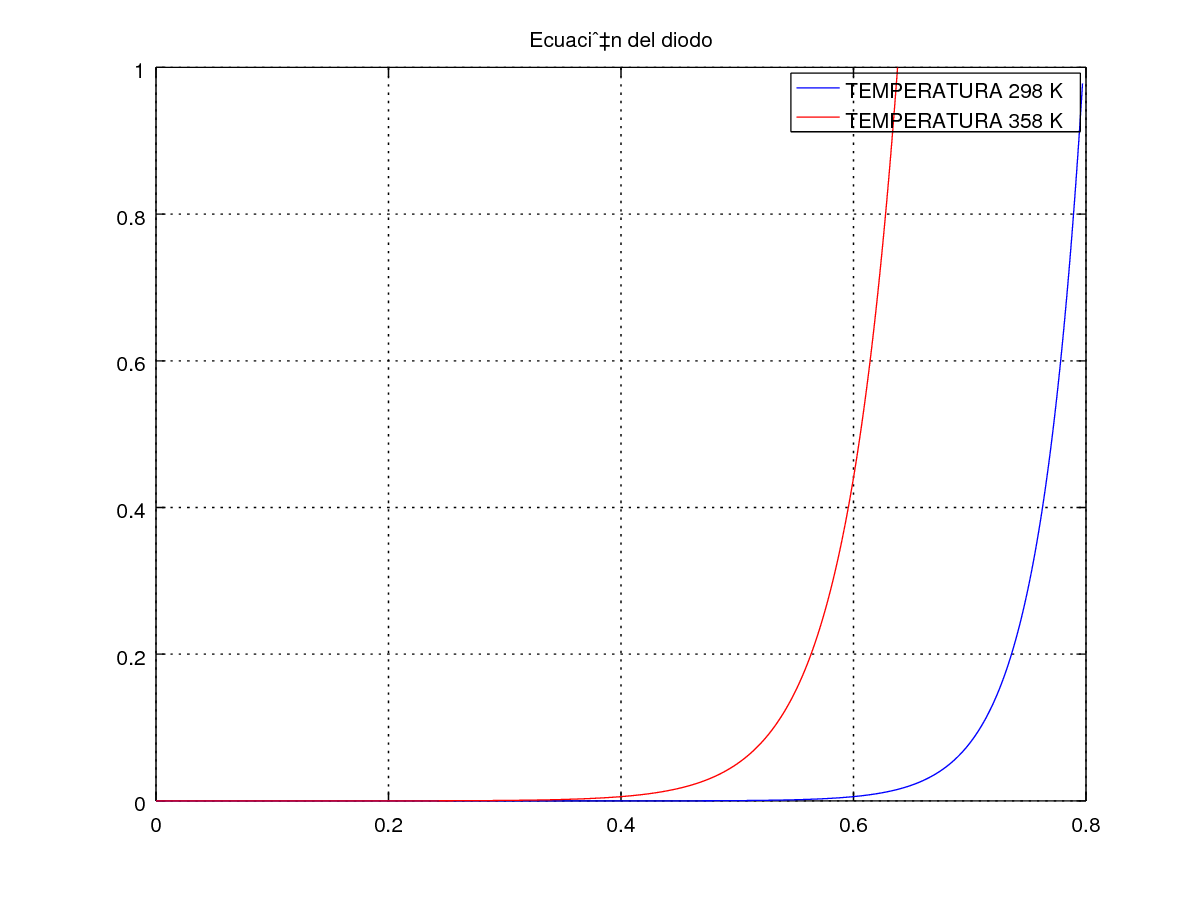
\includegraphics[width=0.6\textwidth]{codigo1.png}
 	\caption{Grafico de Temperaturas}
 	\label{fig:codigo1}
 \end{figure}

\subsection{Descripcion de códigos}

Se describirán línea por línea los siguientes códigos.\\

\subsubsection{Código}

	  \begin{verbatim}
	  k=1.38e-23;
	  \end{verbatim}
	  
	  asignación de una varibale con el nombre $k$ con un valor, la $e$ representa un multiplicador del tipo $x10**$.\\
	  
	  \begin{verbatim}
	  num2=q.*v2;
	   \end{verbatim}
	   
	   Asignación de valor a la variable "num2", que toma como valor la varibale "q" elevada por la variable "v2".\\
	   
	   \begin{verbatim}
	  den2=n*k*w2;
	   \end{verbatim}
	   
	   Asignación de la variable "den" que toma como valor el producto de las variables "n","k" y "w2".\\
	   
	   \begin{verbatim}
	  M2=num2./den2;
	   \end{verbatim}
	   
	   Asignación de la variable "M2" que toma como valor la división de las variables "num2" y "den2".\\
	   
	   \begin{verbatim}
	  x2=1024e-9.*exp(M2);
	   \end{verbatim}
	   
	   Asignación de la variable "x2" que toma como valor 1024 por 10 a la -9, multiplicado por una exponencial elevada a la varibale "M2".\\
	   
	   \begin{verbatim}
	  plot(v1,x1,'b',v2,x2,'r');title('Ecuación del diodo');
	   \end{verbatim}
	   
	   Se graficarán dos funciones, tomando como dominios "v1" y "v2" y como codominios "x1" y "x2", asignándoles como colores azul "b" y rojo "r", se le añadirá un título.\\ 
	   
	   \begin{verbatim}
	    legend('TEMPERATURA 298 K', 'TEMPERATURA 358 K');
	    \end{verbatim}
	    
	    Se añaden etiquetas a cada función
	    
	    \begin{verbatim}
	    grid 
	   \end{verbatim}
	   
	   Se agrega una rejilla a la gráfica.\\
	   
\subsubsection{Código}

  \begin{verbatim}
f=2;
\end{verbatim}

   Asignación de la variable "f" que toma como valor 2.\\

  \begin{verbatim}
w=2*pi*f;
\end{verbatim}

 Asignación de la variable "w" que toma como valor el producto de 2 cn la variable "pi" y "f".\\

  \begin{verbatim}
subplot(2,2,1);plot(t,x,'r','linewidth',2);grid
\end{verbatim}

Declaración de una subgráfica que toma como dominio "t" como codominio "x" y se la agrega una rejilla.\\

  \begin{verbatim}
subplot(2,2,4);loglog(t,x,'b','linewidth',2);grid
\end{verbatim}

Declaración de una subgráfica que toma como dominio "t" como codominio "b" y se la agrega una rejilla.\\

\subsubsection{Código}

\begin{verbatim}
x3=4.*sin(w3.*t);
\end{verbatim}
Asignación de una función a la variable "x3".\\

\begin{verbatim}
plot(t,x1,'b',t,x2,'r',t,x3,'k','linewidth',2);
\end{verbatim}
Declaración de una gráfica múltiple que toma como dominio "t" como codominios "x1","x2" y "x3", se le asignan diferentes colores y un tipo de línea.\\


\begin{verbatim}
title('Cada senoidal completa un numero entero de ciclos');
\end{verbatim}
Se le agrega un título a la gráfica

\begin{verbatim}
grid
\end{verbatim}
Se la agrega una rejilla.

\subsubsection{Código}

\begin{verbatim}
rho(3,:) = sin(theta).^2;
\end{verbatim}
Asignación de una función a la variable "rho".

\begin{verbatim}
rho(4,:) = 5*cos(3.5*theta).^3;
\end{verbatim}
Asignación de una función a la variable "rho".

\begin{verbatim}
for k = 1:4
polar(theta,rho(k,:))           	
end	
\end{verbatim}
Iteraciones con sistintos valores para la variable "rho"

Aunque el código no lo muestre se puede apreciar una gráfica de la función anterior en la figura \ref{fig:petalos}

\begin{figure}[h!]
	\centering
	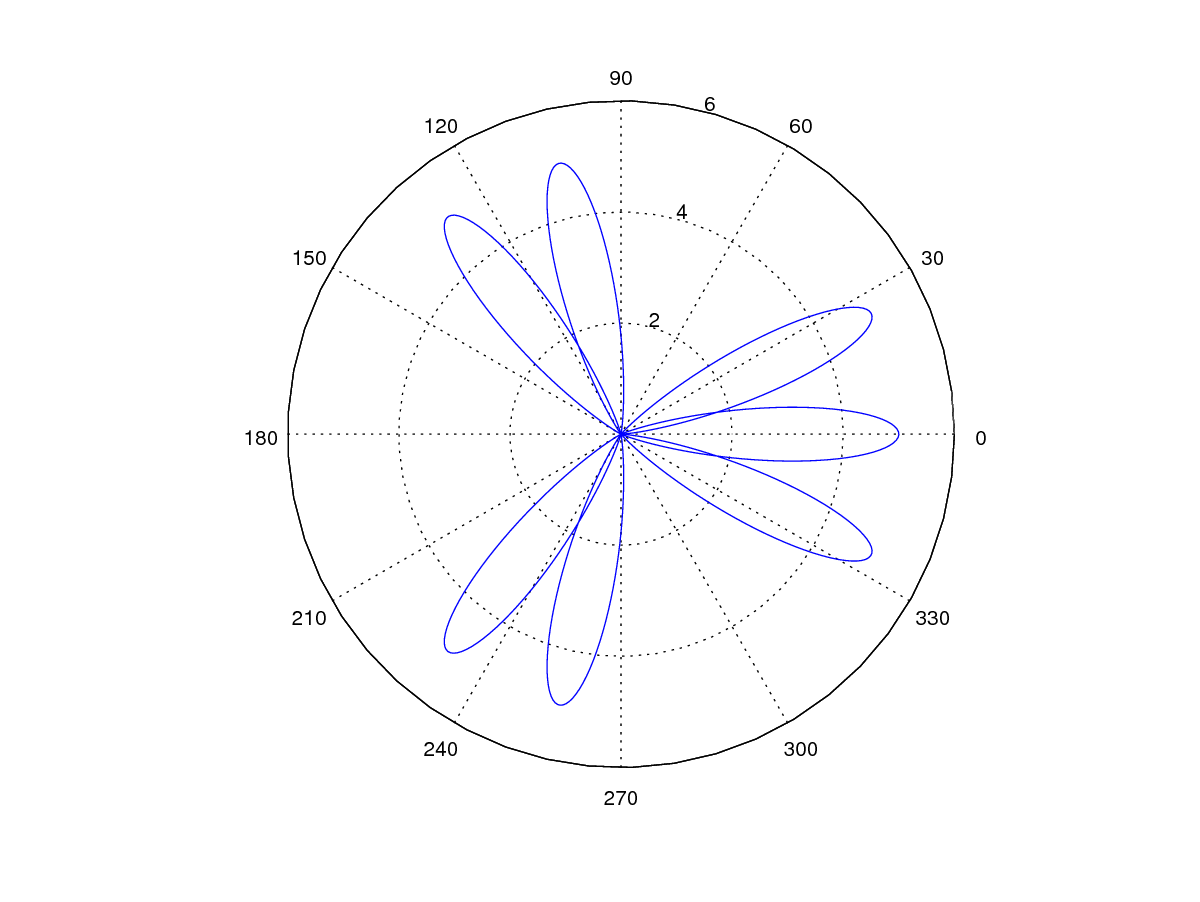
\includegraphics[width=0.6\textwidth]{flor.png}
	\caption{Grafico Polar}
	\label{fig:petalos}
\end{figure}

\section{Análisis de Resultados}

De los códigos anteriormente mostrados, muchos no compilen por si solos, porque hacen falta variables por declarar, éstas variables faltantes se pueden encontrar en el primer código de prueba mostrado, es importante revisar que las variables a utilizar o utilizadas estén previamente declaradas, ya que el programa no podrá trabajar sin ellas.\\

\section{Conclusiones}

Los objetivos generales de la práctica se cumplieron ya que se revisó el manejo de varibales y vectores dentro del entorno de MATLA; también se lograron hacer algunos gráficos, modificar sus parámetros, etc.\\

El objetivo particular se cumplió porque los códigos que compliaron en MATLAB también lo pudieron hacer en GNU/Octave sin ningún inconveniente o realizar ninguna modificación especial lo que demuestra la potencia de ésta plataforma como alternativa a MATLAB.\\

%\bibliographystyle{plain}
%\bibliography{Referencias.bib}
%\addbibresource{Referencias.bib}
\section{Referencias}

\begin{thebibliography}{widestlabel}
	\bibitem{MATLABWiki}\textsc{Wikipedia},\textsc{MATLAB},\textsc{https://en.wikipedia.org/wiki/MATLAB},\textit{},WikimediaGroup.
	
   \bibitem{Deepl}\textsc{Deepl},\textsc{www.DeepL.com/Translator}
	
	
	
\end{thebibliography}


\end{document}
